\documentclass[11pt]{article}

\usepackage{kotex}
\usepackage{graphicx}
\usepackage{gensymb}
\usepackage{subfigure}
\usepackage{floatflt}
\usepackage{wrapfig}
\usepackage{rotating}
\usepackage{psfrag}

\graphicspath{{../images/}}

%\renewcommand{\thesubfigure}{(\hangulb{subfigure})\space}

\begin{document}
Hello World!

\begin{figure}[b]
\centering\includegraphics[scale=0.5]{eps.png}
\caption{\texttt{\symbol{92}includegraphics} 명령으로 부른 그램(축소/확대) \label{fig:eps01}}
\end{figure}

\begin{figure}
\centering\includegraphics[width=.97\textwidth, height=5cm]{eps.png}
\caption{\texttt{\symbol{92}includegraphics} 명령의 그림 크기 조절 \label{fig:eps02}}
\end{figure}

\begin{figure}[t]
\caption{\texttt{\symbol{92}includegraphics}로 그림 일부만 잘라오기 \label{fig:eps03}}
\centering\includegraphics*[300pt, 0pt][600pt, 150pt]{eps.png}
\end{figure}

\begin{figure}[t]
\caption{\texttt{\symbol{92}includegraphics*} 명령의 잘라오기 및 그림 크기 변경 \label{fig:eps04}}
\centering\includegraphics*[bb=300 0 600 150, width=0.5\textwidth, height=0.4\textwidth]{eps.png}
\end{figure}

\begin{figure}[t]
\begin{center}
\includegraphics[width=1.8in]{../images/eps.png}
\includegraphics[width=1.8in, angle=-30]{eps.png}
caption{PostScript 그림 \texttt{eps.png}의 원본 및 반시계 방향으로 30 \degree 회전한 결과 \label{fig:sunrise}}
\end{center}
\end{figure}

\begin{figure}[t]
왼쪽 문자--
\includegraphics*[bb=0 0 150 305]{eps.png}
--오른쪽 문자
\caption{\texttt{*} 있는 \texttt{\symbol{92}includegraphics*} 명령 \label{fig:include*}}
\end{figure}

\begin{figure}[t]
외쪽 문자--
\includegraphics[bb=0 0 150 300]{eps.png}
--오른쪽 문자
\caption{\texttt{*} 없는 \texttt{\symbol{92}includegraphics} 명령 \label{fig:include0}}
\end{figure}

\includegraphics[width=0.5\textwidth, page=5]{style.pdf}

\begin{figure}[!t]
\noindent
\begin{minipage}[t]{2.5in}
\centerline{\includegraphics[width=1.5in, height=1.5in]{eps.png}}
\centerline{(a)원 그래프}
\end{minipage} \hfill
\begin{minipage}[t]{2.5in}
\centerline{\includegraphics[width=1.5in, height=1.5in]{eps.png}}
\centerline{(b)막대 그래프}
\end{minipage}
\caption{원 그래프와 막대 그래프 \label{fig:hist}}
\end{figure}

\begin{minipage}[c]{2.1in}
오른쪽 그림과 같이, 함수 $f(x)=x^3-x^2$의 그래프 위의 점 $(a_0, f(a_0))$에서 접선을 긋고 (단 $a_0>3$) $x$축과의 교점을 $(a_1, 0)$이라 한다. 다음에 점 $(a_1, f(a_1))$에서 접선을 긋고 $x$축과의 교점을 $(a_2, 0)$ 이라 한다. 이러한 방법으로 계속하여 일반적으로 점 $(a_{n-1},f(a_{n-1}))$에서 접선을 긋고 $x$축과의 교점을 $(a_n, 0)$이라 한다. 이때 다음 물음에 답하여라.
\end{minipage}
\  \hfill \
%\begin{minipage}{2.4}
%\begin{tikzpicture}[xscale=2.25,yscale=2.5]
%\draw[thick,->](-0.7,0) -- (1.8,0) node[right] at (1.8,0) {$x$}; % x 축
%\draw[thick,->] (0,-0.5) -- (0,1.5) node[below left] at (0, 1.5) {$y$}; % y 축
%\draw[black, domain=-0.5:1.6] plot (\x, {\x*\x*(\x-1)});
%\draw(1.05, 0) -- (1.2, 0.288) node[below] at (1.05, 0) {\small $a_2$};
%\draw[dotted](1.2, 0.288) -- (1.2, 0);
%\draw (1.2,0) -- (1.5, 1.25) node[right=2mm, below] at (1.2, 0) {\small $a_1$};
%\draw[dotted] (1.5, 1.125) -- (1.5 0) node[below] at (1.5, 0) {\small $a_0$};
%\end{tikzpicture}
%\end{minipage}
\begin{enumerate}
\item $a_n$을 $a_{n_1}$의 식으로 나타내어라$(n=1,2,\cdots)$.
\item $a_0>a_1>a_2>\cdots>a_n>\cdots \geq \sqrt{3}$이 됨을 보여라.
%\item $\dlim{\go \infty}a_n$을 구하여라.
\end{enumerate}

\begin{figure}[!t]
\centerline{
\subfigure[회전]{\includegraphics[width=1.6in,height=2in,angle=45]{eps.png}}
\subfigure[원래 크기]{\includegraphics[width=1.6in,height=2in]{eps.png}} }
\caption{\texttt{subfigure} 패키지를 이요한 그림 1}
\end{figure}

\newpage
\begin{floatingfigure}[b]{80mm}
\fbox{\includegraphics[width=7cm]{eps.png}}
\caption{\mbox{ }\texttt{floatingfigure} 환경의 예 2}
\end{floatingfigure}

Hello wolrd!

\newpage
\clearpage
\begin{floatingtable}
{
\begin{tabular}{|l|p{2.6in}|} \hline
\textit{option} 	& 사용 결과 \\ \hline \hline
\texttt{l} 			& 그림을 왼쪽에 넣을 경우에 설정한다. \\ \hline
\texttt{r}			& 그림을 오른쪽에 넣을 경우에 설정한다. \\ \hline
\texttt{p}			& 그림을 짝수면에는 왼쪽에 홀수면에는 오른쪽에 넣을 경우에 설정한다. (기본값)\\ \hline
\texttt{v}			& \texttt{\symbol{92}usepackage} 명령에서 정해준 옵션을 따른다. \\ \hline
\end{tabular}
}
\caption{\texttt{floatingtable} 환경의 옵}
\end{floatingtable}

Hello world!!!!

\newpage \clearpage
\begin{wraptable}[15]{l}{8cm}
\caption{\texttt{wrapfig}의 \emph{loc} 옵션 \label{tab:wraptable}}
\begin{tabular}{p{2cm}|p{5cm}} \hline
옵션 & 결과 \\ \hline
\texttt{r R} & 텍스트의 오른쪽에 그림이나 표를 만든다. \\
\texttt{l L} & 텍스트의 왼쪽에 그림이나 표를 만든다. \\
\texttt{i I} & 책을 기준으로 책을 펼쳤을 때 그림이 안쪽으로 들어가게 한다. \\
\texttt{o O} & 책을 기준으로 책을 펼쳤을 때 그림이 바깥쪽으로 들어가게 한다. \\ \hline
\end{tabular}
\end{wraptable}

%\begin{wrapfigure}[14]{r}{7cm}
%\caption{\texttt{wrapfigure} 환경으로 만든 \texttt{eps.png}
%\label{fig:wrapfigure}}
%\epsfig{file=eps.png,width=7cm,height=5cm}
%\end{wrapfigure}

\begin{sidewaystable}
\caption[\texttt{rotating} 패키지에서 제공하는 환경] {\texttt{rotating} 패키지에서 제공하는 여러 가지 환경: 이 표는 아래의 \texttt{sidewaystlabe}로 만들었으며 각도는 반시계 방향의 각도이다.
\label{tab:sidewaystable}}
\begin{center}
\begin{tabular}{|l||p{5in}|} \hline
\texttt{sideways} & \verb|\begin{sideways}| 회전할 입력 \verb|\end{sideways}|로 사용하며 주어진 내용을 시계 반대 방향으로 90도 회전시킨다. \\ \hline
\texttt{turn} & \verb|\begin{rotate}{각도}|입력 \verb|\end{rotate}|로 사용한다. \texttt{rotate}도 주어진 내용을 주어진 각도만큼 회전시키는데 공간을 남기지 않는다는 것이다. 따라사 \texttt{turn}과의 차이는 회전 후의 출력을 위한 공간을 남기지 않는다는 것이다. 따라서 \texttt{turn}은 회전할 때 회전에 의해 추가로 만들어야 하는 공간을 고려하지만 \texttt{toatata}는 이를 고려하지 않아 전후좌우의 다른 출력과 겹칠 수 있다. \\ \hline
\texttt{sidewaysfigure} & \verb|\begin{figure}|와 \verb|\end{figure}|의 \texttt{figure} 대신에 \texttt{sidewaysfigure}를 쓰면 그림을 90도 회전시킨다. \\ \hline
\texttt{sidewaystalbe} & \verb|\begin{table}|와 \verb|\end{table}|의 \texttt{table} 대신에 \texttt{sidewaystable}를 쓰면 표를 90도 회전시킨다. \\ \hline
\end{tabular}
\end{center}
\end{sidewaystable}

\begin{center}
---\fbox{\shortstack{\LARGE A B C\\ \LARGE D E F\\
\LARGE G H I}}---
---\begin{turn}{30}
\fbox{\shortstack{\LARGE A B C\\ \LARGE D E F\\ \LARGE G H I}}
\end{turn}---
---\begin{rotate}{30}
\fbox{\shortstack{\LARGE A B C\\ \LARGE D E F\\ \LARGE G H I}}
\end{rotate}---
---\begin{sideways}
\fbox{\shortstack{\LARGE A B C\\ \LARGE D E F\\ \LARGE G H I}}
\end{sideways}---
\end{center}

x <- seq(-3, 6, by=0.1)
y1 <- dnorm(x)
y2 <- dnorm(x-3)

postscript(file="eps.png", width=5, height=4, horizontal=F)
plot(x, y1, type="l", main="title", xlab="x", ylab="y")
lines(x, y2, type="l", lty=3)
text(-2, .2, label="N1")
text(5, .2, label="N2")
graphics.off()

x <- seq(-3, 6, by=0.1)
y1 <- dnorm(x)
y2 <- dnorm(x-3)

postscript(file="eps.png", width=5, height=4, horizontal=F)
plot(x, y1, type="l", main="title", xlab="x", ylab="y")
lines(x, y2, type="l", lty=3)
text(-2, .2, label="N1")
text(5, .2, label="N2")
graphics.off()

\psfrag{title}[][][1.6]
{Compare $\mu=0$ with $\mu=3$ when $\sgima^2=1$}
\psfrag{x}[][][1.3]{$x$축이 한글로}
\psfrag{y}[][][1.3]{$f(x)$}
\psfrag{N1}[][][1.3][75]
{$f(x)=\frac{1}{\sqrt{2\pi}}e^{-\frac{x^2}{2}}$}
\psfrag{N2}[][][1.3][-75]
{$f(x)=\frac{1}{\sqrt{2\pi}}^e{-\frac{(x-3)^2}{2}}$}

\end{document}